% !TeX program = lualatex
\documentclass[]{article}

\usepackage{caption,subcaption,graphicx,float,url,amsmath,amssymb,amsthm,tocloft,cancel,thmtools,gensymb,braket,tikz-feynman,mathtools}
\usepackage[toc,nonumberlist]{glossaries}
\usepackage{glossaries-extra}
\newcommand\numberthis{\addtocounter{equation}{1}\tag{\theequation}}

\newtheorem{thm}{Theorem}
\newtheorem{defn}[thm]{Definition}
\newtheorem{cor}[thm]{Corollary}
\newtheorem{lemma}[thm]{Lemma}
\graphicspath{{figs/}}
\widowpenalty10000
\clubpenalty10000
\setcounter{tocdepth}{2}
\tikzfeynmanset{compat=1.0.0}
%opening
\title{Theoretical Minimum\ Quantum Entanglement}
\author{Simon Crase (compiler)\\simon@greenweaves.nz}

\begin{document}

\maketitle

\begin{abstract}
These are my notes from the Quantum Entanglement lectures\cite{susskind2013entanglement}  from Leonard Susskind's Theoretical Minimum series\cite{susskind2007theoretical}.

Disclaimer: I have created these notes as an aide-m\'emoire for my own use; if you find them useful, you are welcome, but I'd appreciate hearing from you. They are not intended 
as a substitute for listening to the lectures. The intellectual property for all material derived from the lectures belongs, of course, to Professor Susskind; any mistakes, however, are my own.

The notes were created using TexStudio\cite{TexStudio}, which I recommend for compiling them to a PDF, and the bibliography was created using JabRef\cite{Jabref}.

\end{abstract}

\tableofcontents
\listoffigures
\listoftables
\listoftheorems


\section{Introduction}


We, as animals, have inherited, through the process of evolution, certain intuitive ways of thinking about the physical world:
\begin{enumerate}
	\item Lioness pursuing antelope will stop as soon as relative velocity changes sign (physics calculation!);
	\item Neanderthal pushing rock from door of cave aims body to maximize component of force in the right direction.
\end{enumerate}

Everything in modern physics has to do with those things that are beyond these intuitions:
speeds approaching speed of light; 4 D; the electron; the uncertainty principle. Why would natural selecton have given us the intuition of the uncertainty principle? Intuitions for particles come from rocks.

This course will try to expose some of the weirdness of quantum mechanics, the weirdness of the logic quantum mechanics, the weirdness of how quantum information works. 

This course will cover:
\begin{enumerate}
	\item the basic logic of quantum mechanics;
	\item the basic logic of quantum information theory
	\item physics as information.
\end{enumerate}

Classical mechanics represents values as real numbers; QM often uses discrete values. Before we cover quantum bits we will look at classical bits, and we will use Dirac's notation\cite{susskind2014quantum} $\ket{0}$ or $\ket{1}$\cite{susskind2014quantum}. For an $n-bit$ \emph{classical} system, the number of configurations is $N_S=2^n$, so $n=\log_2(N_S)$.

We can generalize definition of number of bits of information: it doesn't have to be an integer. We can represent the state of a physical system, to specified precision, by a string of bits (quantize space, etc). Figure \ref{fig:state_transition} shows how the laws of physics can be represented as a state transition diagram.

\begin{figure}[H]
	\caption{The laws of physics can be represented as a state transition diagram. In quantum mechanics there is no fundamental difference between forward in time and backward in time.}\label{fig:state_transition}
	\begin{subfigure}[t]{0.45\textwidth}
		\caption{Reversible Laws}\label{fig:state_transition_reversible}
		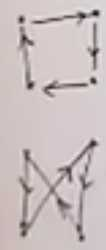
\includegraphics[width=0.8\textwidth]{et-1-1}
	\end{subfigure}
	\begin{subfigure}[t]{0.45\textwidth}
		\caption{An irreversible law}
		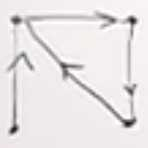
\includegraphics[width=0.8\textwidth]{et-1-2}
	\end{subfigure}
\end{figure}

All real systems are quantum mechanical. In this course we will try to answer the question why the quantum mechanics is suppressed in many systems we observe.

A Newtonian system is one that is in a definite state, and that evolves deterministically.

Second Law of Thermodynamics arises because we lose the ability to follow the evolution of a system in precise detail.

Review of vectors and matrices:
\begin{itemize}
	\item Row and column vectors as sequences of number;
	\item Inner products;
	\item Matrices--linear transformation of vectors.
\end{itemize}

We can represent a state by a "one hot" vector, and then represent the transitions of, say, Figure \ref{fig:state_transition_reversible}, by a matrix of ones and zeros.

\section{Quantum Entanglement}

\section{Quantum Entanglement}

\section{Quantum Entanglement}

\section{Quantum Entanglement}

\section{Quantum Entanglement}

\section{Quantum Entanglement}

\section{Quantum Entanglement}

\section{Quantum Entanglement}

\bibliographystyle{unsrt}
\addcontentsline{toc}{section}{Bibliography}
\raggedright
\bibliography{tm}

\end{document}